\documentclass[12pt]{article} % document type and language

\usepackage{amsmath, amssymb, bm, mathtools, cancel, empheq, ulem, mathrsfs, natbib}
\setcitestyle{aysep={}} 
%\usepackage{newtxmath} 
\usepackage[margin=1in]{geometry}

\usepackage[colorlinks]{hyperref}
\hypersetup{
	colorlinks = true,
	linkcolor=blue,
	citecolor=blue
}

% Allow option to set color when hyperlinking
\newcommand{\MYhref}[3][blue]{\href{#2}{\color{#1}{#3}}}

\date{\today}
\author{Loren Matilsky}
\title{Angular Momentum in Terms of Toroidal and Poloidal Stream Functions}

\input ../macros.tex

\allowdisplaybreaks
\begin{document}
	\maketitle

\section{Prior Work Considered}
In this set of notes, we consider 3D nonlinear dynamo simulations that explored magnetic-field amplitudes at a variety of rotation rates (i.e., enough to make scatter plots of various quantities versus Rossby number and thus theoretically address the activity-rotation relation). We aim to determine what region of parameter space has been explored by global models, and in particular, how the rotation-activity relation may or may not have been addressed. The works considered are:\\

\citet{Christensen2006},\\

\citet{Christensen2009},\\

\citet{Strugarek2017},\\

\citet{Guerrero2019},\\

\citet{Brun2022},\\

\section{Observations of the Stellar Activity-Rotation Relation (ARR)}
The stellar activity-rotation relation (hereafter ARR) has a long history of observation and informs astronomers' generally accepted picture of stellar spin-down. The fact that rotational velocity ($v\sin i$) and chromospheric $\text{Ca}^+$ emission (believed to be linearly proportional to the surface magnetic field) are positively correlated was first noted by \citet{Kraft1967}. This correlation was made famous (in the context of spin-down) by the ``Skumanich $t^{1/2}$" law. This law states that as a star ages (call its age $t$), its surface magnetic-field strength and rotation rate both decrease like $t^{-1/2}$ \citep{Skumanich1972}. Since spin-down is believed to be caused by angular-momentum loss from a stellar wind, there appears to be a negative feedback loop between rotation (which produces magnetic field by a convective dynamo) and magnetic field (which drives the stellar wind and slows the rotation). 

In addition to chromospheric emission, coronal emission (X-ray luminosity) is also found to be proportional to rotation rate (e.g., \citealt{Walter1982}). The X-ray data also showed that for a critical rotation rate (corresponding to a critical mixing-length Rossby number of $Ro\sim0.1$), the ratio of X-ray luminosity to total luminosity saturated to a value of $\sim0.001$. It is still unclear whether this saturation regime corresponds a fundamental dynamo process (for example, the inability of the dynamo to convert additional rotational energy to magnetic field) or simply geometric effects (for example, the stellar surface becoming so peppered with active regions that it cannot accommodate any more dynamo-produced flux) \citep{Jardine1999}. 

 \citet{Reiners2022} has the most recent description of the ARR we are aware of. Figure \ref{fig:arr} shows the ARR as reported by \citet{Reiners2022}. As the Rossby number $Ro$ (ratio of rotation period to convective turnover time) decreases right to left (i.e., the rotation rate increases), the surface magnetic field strength increases up to a critical Rossby number $Ro=0.13$. After that, faster rotation only leads to marginally increased field strength; this regime of dynamos in fast-rotating systems is known as the ``saturation regime."

\begin{figure*}\label{fig:arr}
	\centering
	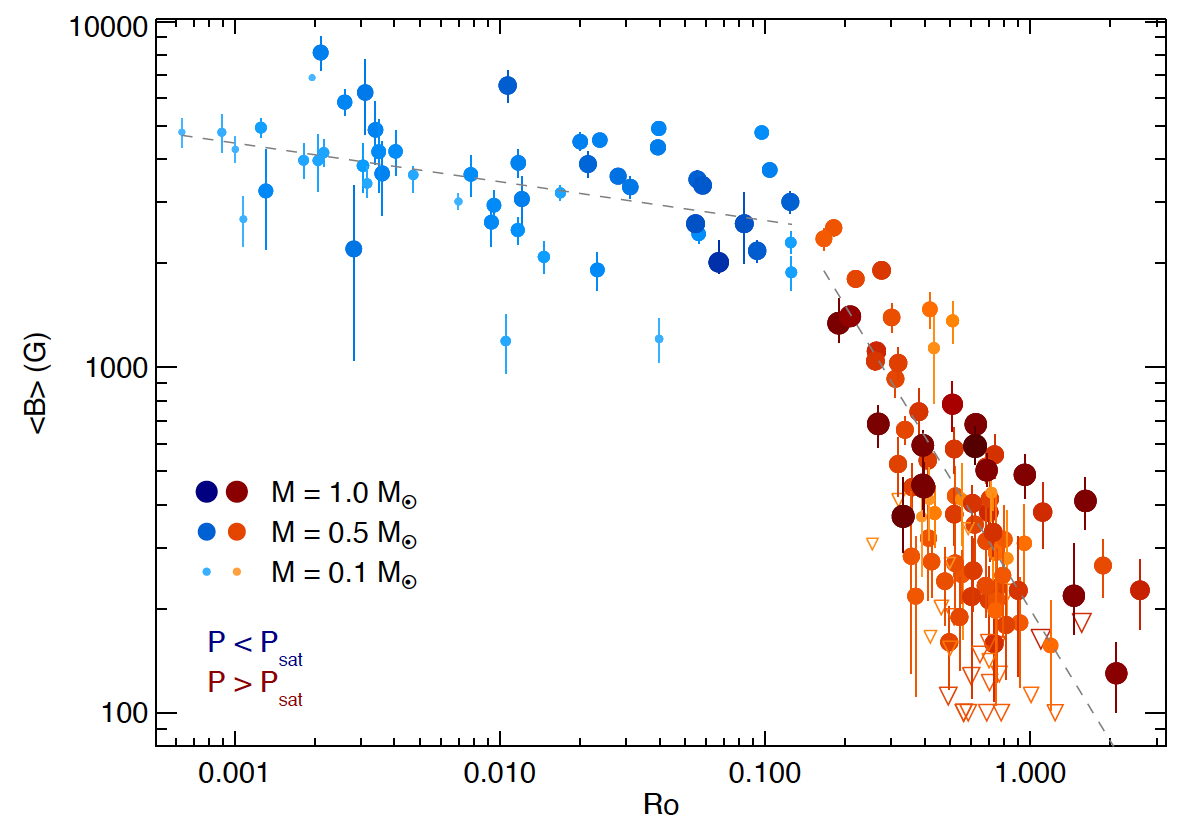
\includegraphics[width=6.5in]{ARR.png}
	\caption{Copied from \citet{Reiners2022}, Figure 5: Magnetic field–rotation relation for solar-like and low-mass stars. Symbols for stars rotating slower than $Ro=0.13$ are colored red, while those of faster rotators are colored blue. Larger and darker symbols indicate higher stellar mass than smaller and lighter symbols.  The gray dashed lines show linear fits separately for the slowly rotating stars ($Ro>0.13$;  $\av{B}=200G\times Ro^{-1.25}$) and the fast rotators ($Ro<0.13$; $\av{B}=2050 G \times Ro^{-0.11}$). Downward open triangles show upper limits for $\av{B}$.}
\end{figure*}

Historical 

	\bibliography{/Users/loren/Desktop/Paper_Library/000_bibtex/library_propstyle,
	/Users/loren/Desktop/Paper_Library/000_bibtex/proceedings,
	/Users/loren/Desktop/Paper_Library/000_bibtex/books}
\bibliographystyle{../aasjournal2}

\end{document}